%---------------------------------------------------------------------------------------------------------
%---------------------------------------------------------------------------------------------------------
\section{Introduction}

Nous allons dans cette partie voir une m\'ethode de r\'esolution num\'erique d'un probl\`eme simple de
contr\^ole optimal utilisant les conditions n\'ecessaires d'optimalit\'e, c'est-\`a-dire le Principe
du Maximum de Pontryagin (PMP). Cette m\'ethode fait partie des m\'ethodes dites indirectes et s'appelle
la m\'ethode de tir simple.
%Vous pouvez consulter la r\'ef\'erence suivante pour une description
%des diff\'erentes m\'ethodes num\'eriques de r\'esolution de probl\`emes de contr\^ole optimal~: A.~V.~Rao,
%\emph{A survey of numerical methods for optimal control}.

%---------------------------------------------------------------------------------------------------------
%---------------------------------------------------------------------------------------------------------
\section{Pr\'esentation de la m\'ethode de tir simple sur un exemple}

\subsection{Le probl\`eme de contr\^ole optimal}

    Consid\'erons le probl\`eme de contr\^ole optimal suivant.
    \leqnomode
    \begin{equation}
    \tagProblem
        \left\{ 
            \begin{array}{l}
                \displaystyle J(u(\cdot))  \coloneqq \displaystyle \frac{1}{2} \int_0^{t_f} u(t)^2 \, \diff t\longrightarrow \min \\[1.0em]
                \dot{x}(t)                      =  \displaystyle -x(t)+u(t), \quad  u(t) \in \R, \quad t \in \intervalleff{0}{t_f} \text{ p.p.}, \\[1.0em]
                x(0) = x_0 , \quad x(t_f) = x_f,
            \end{array}
        \right. 
        \label{eq:ocpSimple}
    \end{equation}
    \reqnomode
    avec $t_f \coloneqq 1$, $x_0 \coloneqq -1$, $x_f \coloneqq 0$ et $\forall\, t \in\intervalleff{0}{t_f}$, $x(t) \in \R$.
    Notons 
    \[
        H(x,p,p^0,u) \coloneqq p \, (-x+u) + p^0\, \frac{1}{2} u^2,
    \]
    le pseudo-hamiltonien associ\'e au probl\`eme \eqref{eq:ocpSimple}.

\subsection{Application du principe du maximum de Pontryagin}

    D'apr\`es le PMP, si $u(\cdot)$ est une solution optimal de \eqref{eq:ocpSimple} (avec $x(\cdot)$ la trajectoire associ\'ee)
    alors il existe un vecteur adjoint $p(\cdot) \in AC(\intervalleff{0}{t_f},\R)$, un scalaire $p^0 \le 0$, tels que $(p(\cdot),p^0) \ne (0,0)$,
    et tels que les \'equations suivantes sont v\'erifi\'ees pour $t\in\intervalleff{0}{t_f}$ p.p. :
    \begin{equation*}
        \left\{ 
            \begin{array}{ll}
                \dot{x}(t)  & = \phantom{-} \partial_p H[t] = -x(t)+u(t),   \\[0.5em]
                \dot{p}(t)  & = -           \partial_x H[t] = p(t),         \\[0.5em]
                0           & = \phantom{-} \partial_u H[t] = p(t)+p^0 u(t),
            \end{array}
        \right. 
    \end{equation*}
    o\`u $[t] := (x(t),p(t),p^0,u(t))$.
    Il n'y a pas d'anormale car si $p^0=0$ alors $p(\cdot)\equiv0$ ce qui est impossible. Ainsi, on a $p^0 < 0$.

    \begin{myQuestion}
        \label{question:hamiltonien}
        %\begin{Question}
            Expliquer pourquoi la condition de maximisation du hamiltonien donn\'ee par le PMP :
            \begin{equation*}
                H[t] = \max_{w\in\R} H(x(t),p(t),p^0,w),
            \end{equation*}
            est \'equivalente dans cet exemple \`a la condition :
            \begin{equation*}
                0 = \partial_u H[t].
            \end{equation*}
        %\end{Question}
    \end{myQuestion}

    Notons 
    $
        u_s(x,p,p^0) \coloneqq - p/p^0,
    $
    la solution de l'\'equation $0 = \partial_u H(x,p,p^0,u)$ pour $(x,p,p^0)$ fix\'e.
    On peut alors fixer arbitrairement $p^0\ne 0$ car pour tout $\alpha \in \Rs$, $u_s(x,\alpha p, \alpha p^0) = u_s(x,p,p^0)$ et la trajectoire
    associ\'ee reste inchang\'ee. Fixons $p^0 = -1$ et notons maintenant
    \begin{equation}
        u_s(x,p) = p
        \label{eq:controleOCPSimple}
    \end{equation}
    le contr\^ole optimal.

\subsection{Probl\`eme aux deux bouts}

L'application du PMP nous m\`ene \`a r\'esoudre le \emph{probl\`eme aux deux bouts} (Two Points Boundary Value Problem) suivant~:
    \leqnomode
    \begin{equation}
    \tagProblem
        \left\{ 
            \begin{array}{ll}
                \dot{x}(t)  & = -x(t) + u_s(x(t),p(t)) = -x(t)+p(t),              \\[0.5em]
                \dot{p}(t)  & = \phantom{-}p(t),                                    \\[0.5em]
                x(0)        & = x_0, \quad x(t_f) = x_f.
            \end{array}
        \right. 
        \label{eq:bvpSimple}
    \end{equation}
    \reqnomode
    L'inconnue de ce probl\`eme aux deux bouts est le vecteur adjoint initial $p(0)$.
    En effet si l'on fixe $p(0) \eqqcolon p_0$ alors d'apr\`es le th\'eor\`eme de Cauchy--Lipschitz, il existe une unique solution maximale
    $z(\cdot)\coloneqq(x(\cdot),p(\cdot))$ v\'erifiant la dynamique (sur $x$ et $p$) et la condition initiale $z(0) = (x_0,p_0)$.
    Le probl\`eme est donc de trouver $p_0$ tel que $x(t_f) = x_f$.

\subsection{Fonction de tir et m\'ethode de tir (simple)}

    On va transformer le probl\`eme aux deux bouts \eqref{eq:bvpSimple} en un syt\`eme d'\'equations non lin\'eaires, que l'on appelle \'equations de tir.
    Pour cela, on d\'efinit tout d'abord le syst\`eme hamiltonien 
    \begin{equation}
        \vvec{H}(x,p) \coloneqq \left( \frp{H}{p}(x,p,u_s(x,p)), -\frp{H}{x}(x,p,u_s(x,p)) \right).
        \label{eq:sysHamTirSimple}
    \end{equation}
    %
    On note alors $z \coloneqq (x,p)$, puis $z(\cdot,x_0,p_0)$ la solution de l'\'equation diff\'erentielle $\dot{z}(t) = \vvec{H}(z(t))$
    v\'erifiant $z(0,x_0,p_0) = (x_0,p_0)$.
    %
    On d\'efinit enfin la \emph{fonction de tir} suivante :
    \begin{equation}
        \begin{array}{rlll}
            S \colon    & \R    & \longrightarrow   & \R \\
                        & y     & \longmapsto       & S(y) \coloneqq \Pi_x(z(t_f,x_0,y)) - x_f,
        \end{array}
        \label{eq:fonctionDeTirSimple}
    \end{equation}
    o\`u $\Pi_x$ est simplement la projection canonique $\Pi_x(x,p) = x$.
    %
    R\'esoudre le probl\`eme aux deux bouts \eqref{eq:bvpSimple} revient \`a trouver un z\'ero de la fonction de tir, 
    \ie consiste \`a r\'esoudre
    \begin{equation}
        S(y) = 0.
        \label{eq:eqTirSimple}
    \end{equation}
    La \emph{m\'ethode de tir simple} consiste \`a r\'esoudre les \'equations non lin\'eaires \eqref{eq:eqTirSimple}. On utilise pour cela une m\'ethode 
    de type Newton. Pour augmenter l'efficacit\'e de l'algorithme, nous pouvons fournir la jacobienne de la fonction de tir,
    \cf sujet \ref{chap:jacobienne_tir_simple}.

    \begin{myremark}
        \anoter
        Si $\psol_0$ v\'erifie $S(\psol_0)=0$, alors 
        la courbe int\'egrale $\zsol(\cdot)$ solution de l'\'equation diff\'erentielle $\dot{z}(t) = \vvec{H}(z(t))$, $z(0) = (x_0,\psol_0)$,
        avec le contr\^ole $\usol(\cdot) \coloneqq u_s(\zsol(\cdot))$,
        est une BC-extr\'emale du probl\`eme \eqref{eq:ocpSimple}, \ie cette extr\'emale satisfait les conditions n\'ecessaires d'optimalit\'e
        donn\'ees par le PMP.
    \end{myremark}

\subsection{Calcul du z\'ero de la fonction de tir}

    Calculons la solution \`a la main sur cet exemple simple.
    \[
        \dot{p}(t) = p(t) \Longrightarrow p(t) = e^t \, p_0,~ p_0 \coloneqq p(0) \Longrightarrow x(t) = (0.5\, p_0 \,e^{2\,t} + C)\, e^{-t},~ C \in \R.
    \]
    Or $x(0) = x_0$ donc 
    \[
        x(t) = (0.5\, p_0 \, (e^{2\,t} - 1) + x_0 )\, e^{-t}
    \]
    et finalement, puisque $x_0 = -1$, $x(t_f) = x_f = 0$ et $t_f = 1$, on a
    \[
        \psol_0 = \frac{2 \, (x_f \, e^{t_f} - x_0)}{e^{2\,t_f}-1} = \frac{2}{e^{2}-1} \approx 0.313.
    \]

%---------------------------------------------------------------------------------------------------------
%---------------------------------------------------------------------------------------------------------
\section{Impl\'ementation \matlab\ de la m\'ethode de tir simple}

L'objectif est d'\'etudier le probl\`eme \eqref{eq:ocpSimple} pour retrouver les r\'esultats de la
figure \ref{fig:results_tests_tir_simple}.

\begin{figure}[ht!]
    \begin{center}
        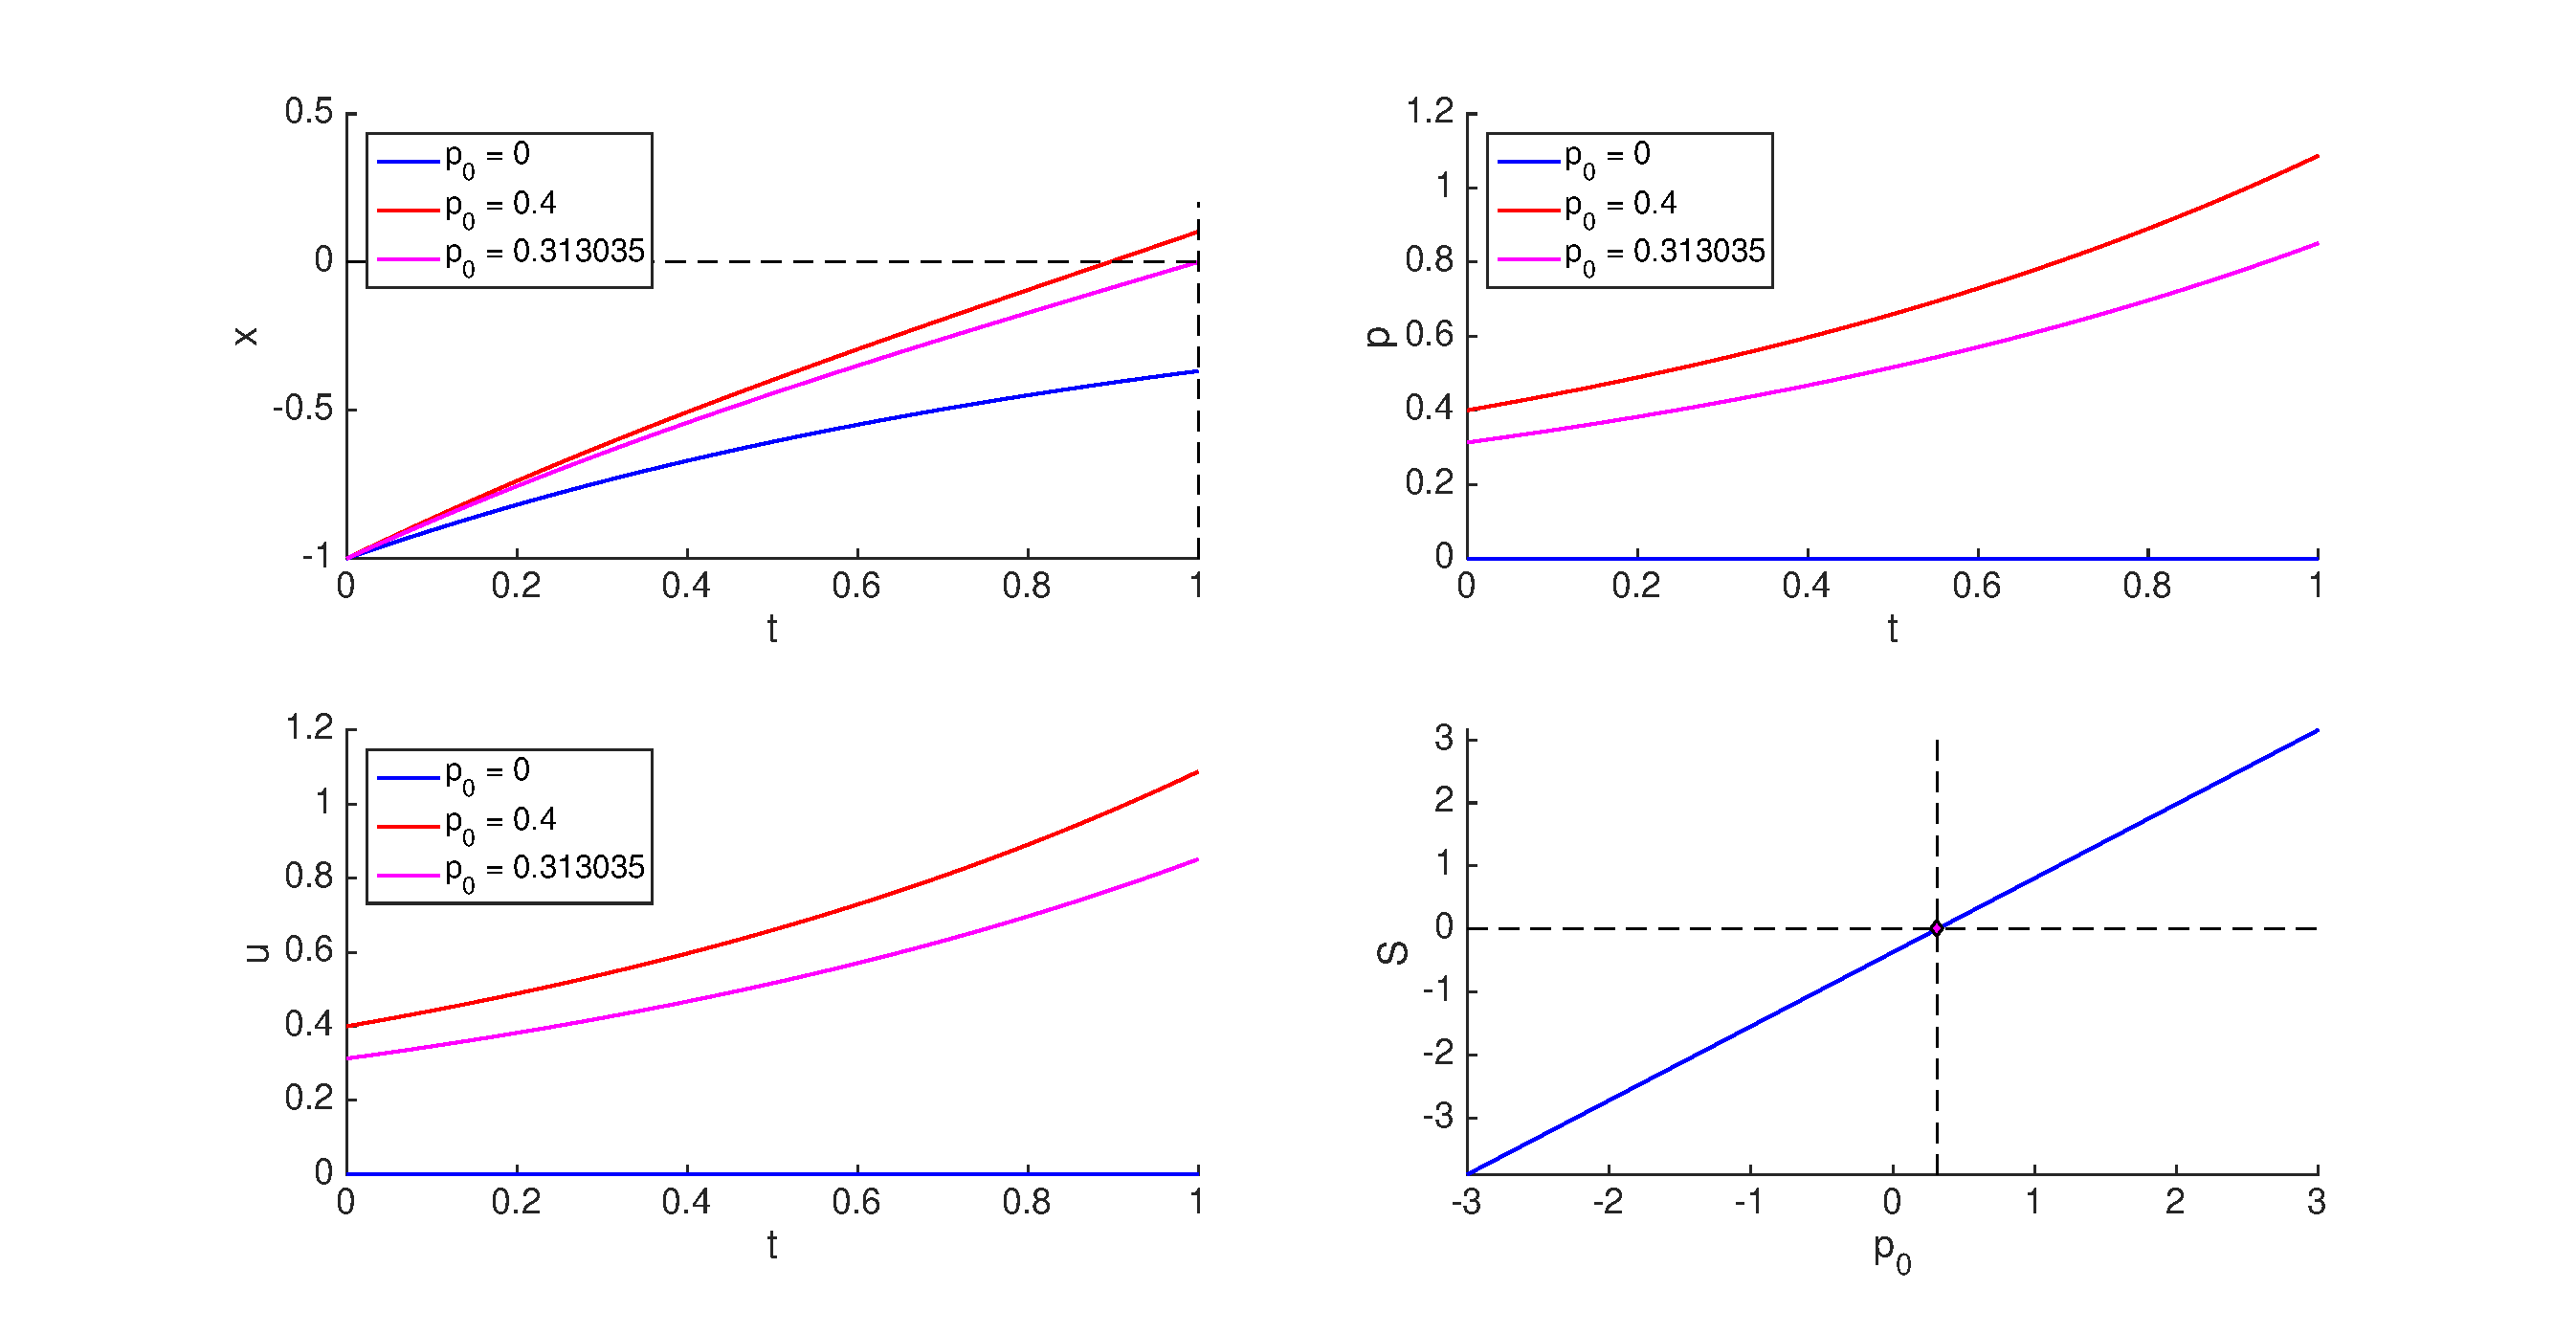
\includegraphics[width=0.9\textwidth]{results_tests_tir_simple}
    \end{center}
    \caption{R\'esultats apr\`es ex\'ecution du fichier \cmd{sujet1\_tir\_simple/probleme1/main.m}.}
    \label{fig:results_tests_tir_simple}
\end{figure}

%------------------------------------------------
\subsection{Le syst\`eme hamiltonien}

\begin{myExercice} Impl\'ementation du syst\`eme hamiltonien.
\begin{enumerate}
    \item Se rendre dans le r\'epertoire \cmd{sujet1\_tir\_simple/probleme1}.
    \item Compl\'eter le fichier \cmd{lib/control.m} qui code le contr\^ole, \cf \'eq.~\eqref{eq:controleOCPSimple}.
    \item Compl\'eter le fichier \cmd{lib/hvfun.m} qui code le syst\`eme hamiltonien, \cf \'eq.~\eqref{eq:sysHamTirSimple}.
    \item Lancer le script \cmd{main.m} et v\'erifier le code de \cmd{lib/hvfun.m}.
\end{enumerate}
\end{myExercice}

%------------------------------------------------
\subsection{Int\'egration num\'erique du syst\`eme hamiltonien}

\begin{myExercice} Int\'egration num\'erique du syst\`eme hamiltonien.
\begin{enumerate}
    \item Compl\'eter le fichier \cmd{lib/exphvfun.m} qui permet le calcul de la solution de l'\'equation diff\'erentielle
        $\dot{z}(t) = \vvec{H}(z(t))$, $z(0) = z_0$.
        \begin{itemize}
            \item Utiliser un ``Function Handle'', voir ``Creating a Function Handle'' sur la documentation de \matlab.
            \item Utiliser la fonction \matlab\ \cmd{ode45.m} (voir \cmd{>> doc ode45}).
        \end{itemize}
        Attention, les fonctions \cmd{ode45} et \cmd{exphvfun} ne renvoient pas les m\^emes types de donn\'ees en sortie.
    \item Lancer le script \cmd{main.m} et v\'erifier le code de \cmd{lib/exphvfun.m}.
\end{enumerate}
\end{myExercice}

\begin{myremark}
    La notation \cmd{exphvfun} vient de la notation math\'ematique suivante :
    \[
        \expmap{z_0}{t_f}{\vvec{H}} \coloneqq z(t_f,z_0),
    \]
    o\`u $z(\cdot,z_0)$ est la solution de l'\'equation diff\'erentielle $\dot{z}(t) = \vvec{H}(z(t))$, $z(0) = z_0$.
\end{myremark}

%------------------------------------------------
\subsection{Fonction de tir}

\begin{myExercice} Impl\'ementation de la fonction de tir.
\begin{enumerate}
    \item Compl\'eter le fichier \cmd{lib/sfun.m} qui code la fonction de tir \eqref{eq:fonctionDeTirSimple}.
    \item Lancer le script \cmd{main.m} et v\'erifier le code de \cmd{lib/sfun.m}.
\end{enumerate}
\end{myExercice}

%------------------------------------------------
%\subsection{Rappel sur la m\'ethode de Newton}

%------------------------------------------------
\subsection{M\'ethode de tir simple}

\begin{myExercice} Impl\'ementation de la m\'ethode de tir et r\'esolution des \'equations de tir.
\begin{enumerate}
    \item Compl\'eter le fichier \cmd{lib/ssolve.m} qui code la m\'ethode de tir, pour r\'esoudre l'\'equation \eqref{eq:eqTirSimple}.
        Utiliser la fonction \matlab\ \cmd{fsolve.m} (voir \cmd{>> doc fsolve}) et un ``Function Handle''.
    \item Lancer le script \cmd{main.m} et v\'erifier le code de \cmd{lib/ssolve.m}.
\end{enumerate}
\end{myExercice}

%---------------------------------------------------------------------------------------------------------
%---------------------------------------------------------------------------------------------------------
\section{Convergence de la m\'ethode de tir}

L'objectif est d'analyser une cause de non convergence de la m\'ethode de tir et de retrouver les r\'esultats de la
figure \ref{fig:results_tests_tir_simple_contraint}.

\begin{figure}[ht!]
    \begin{center}
        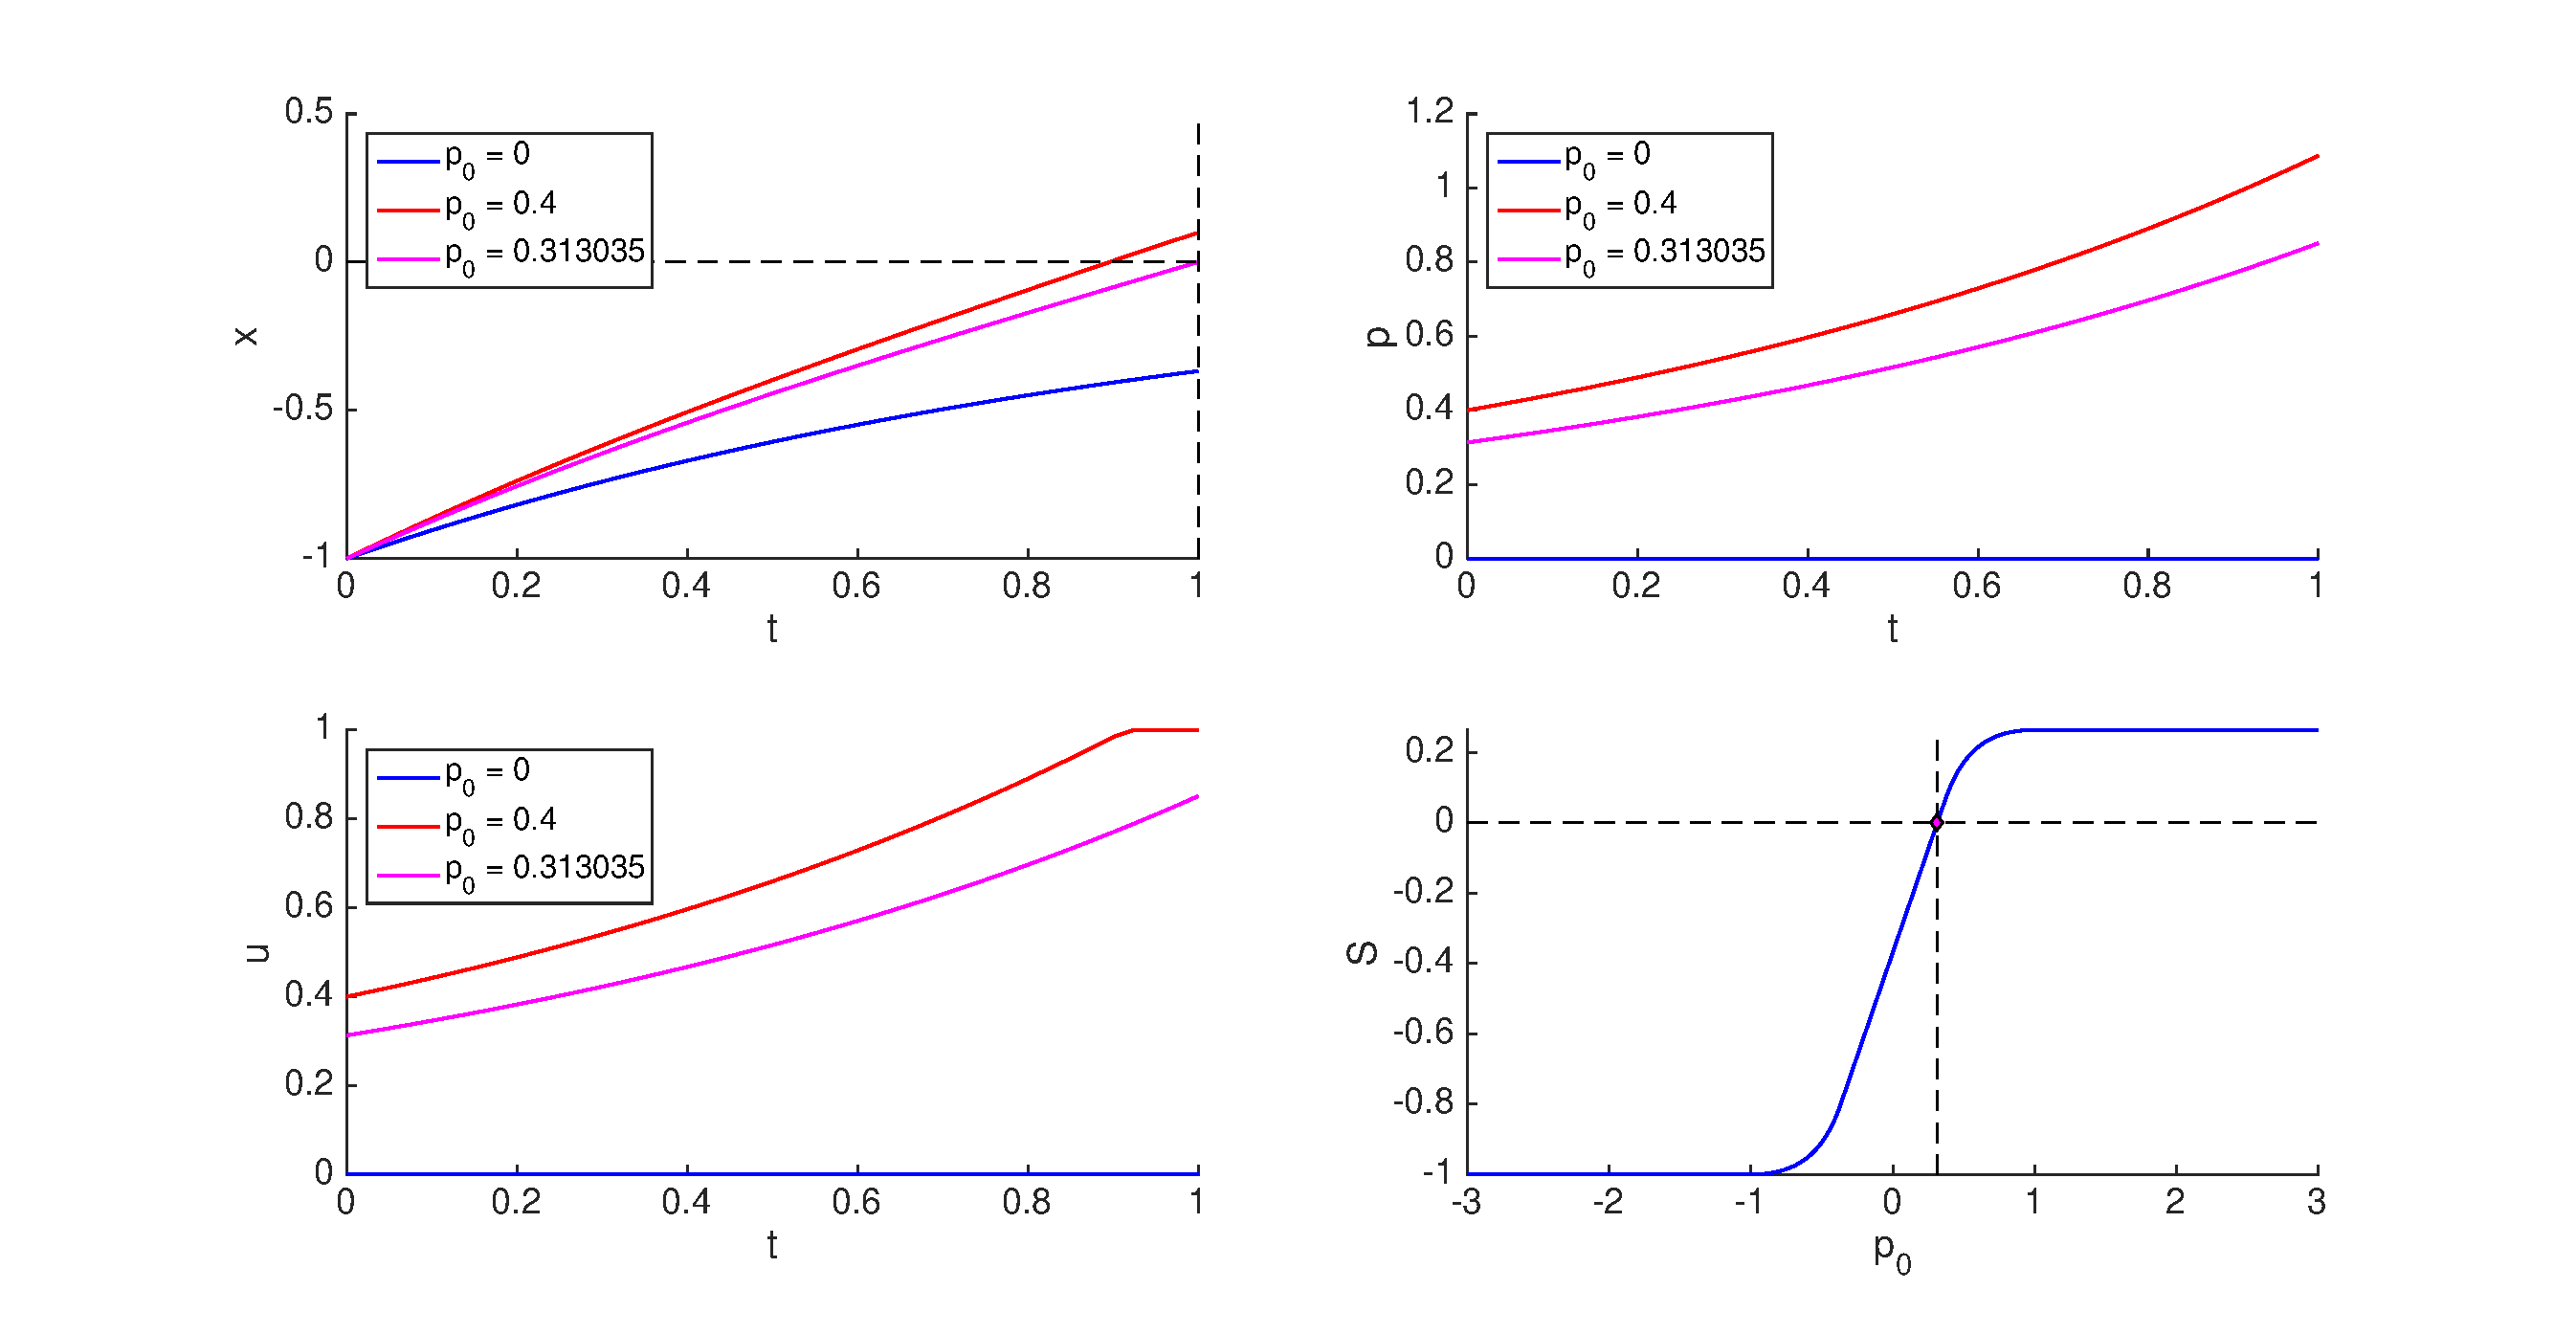
\includegraphics[width=0.95\textwidth]{results_tests_tir_simple_contraint}
    \end{center}
    \caption{R\'esultats apr\`es ex\'ecution du fichier \cmd{sujet1\_tir\_simple/probleme2/main.m}.}
    \label{fig:results_tests_tir_simple_contraint}
\end{figure}

\subsection{Probl\`eme avec contraintes sur le contr\^ole}

On consid\`ere le probl\`eme de contr\^ole \eqref{eq:ocpSimple} o\`u l'on remplace la contrainte sur le contr\^ole par
$u(t) \in \intervalleff{-1}{1}$. La condition de maximisation nous donne comme loi de contr\^ole~:
\begin{equation}
    \tag{\ref{eq:controleOCPSimple}$^*$}
    u(t) = 
    \left\{
        \begin{array}{ll}
            u_s(x(t),p(t)) = p(t)   & \text{ si } \abs{p(t)} \le 1, \\[0.5em]
            +1                      & \text{ si } p(t) > 1, \\[0.5em]
            -1                      & \text{ si } p(t) < -1.
        \end{array}
    \right.
    \label{eq:controleOCPSimpleContraint}
\end{equation}

\subsection{R\'esolution des \'equations de tir et influence du point initial}

\begin{myExercice} R\'esolution des \'equations de tir.
    \begin{enumerate}
        \item Se rendre dans le r\'epertoire \cmd{sujet1\_tir\_simple/probleme2}.
        \item Impl\'ementer dans le r\'epertoire \cmd{lib} les fonctions \cmd{control} (qui code \eqref{eq:controleOCPSimpleContraint}),
            \cmd{hvfun}, \cmd{exphvfun}, \cmd{sfun} et \cmd{ssolve}.
        \item Ex\'ecuter le script \cmd{main.m} et v\'erifier les r\'esultats.
        \item V\'erifier que la m\'ethode de tir ne converge pas si l'on donne comme point initial \`a l'algorithme~: $y^{(0)} = 1.5$.
    \end{enumerate}
\end{myExercice}

\begin{myQuestion}
    \label{question:tir_simple}
    Expliquer pourquoi la m\'ethode de tir ne converge pas pour $y^{(0)} = 1.5$.
\end{myQuestion}

%---------------------------------------------------------------------------------------------------------
%---------------------------------------------------------------------------------------------------------
\section{Probl\`eme en dimension 2 avec contraintes sur le contr\^ole}

L'objectif est dans un premier temps, de retrouver les r\'esultats de la figure \ref{fig:results_tests_tir_simple_dim2}, puis
d'\'etudier l'influence des contraintes sur le contr\^ole pour un probl\`eme avec un crit\`ere quadratique en le contr\^ole.

\begin{figure}[ht!]
    \begin{center}
        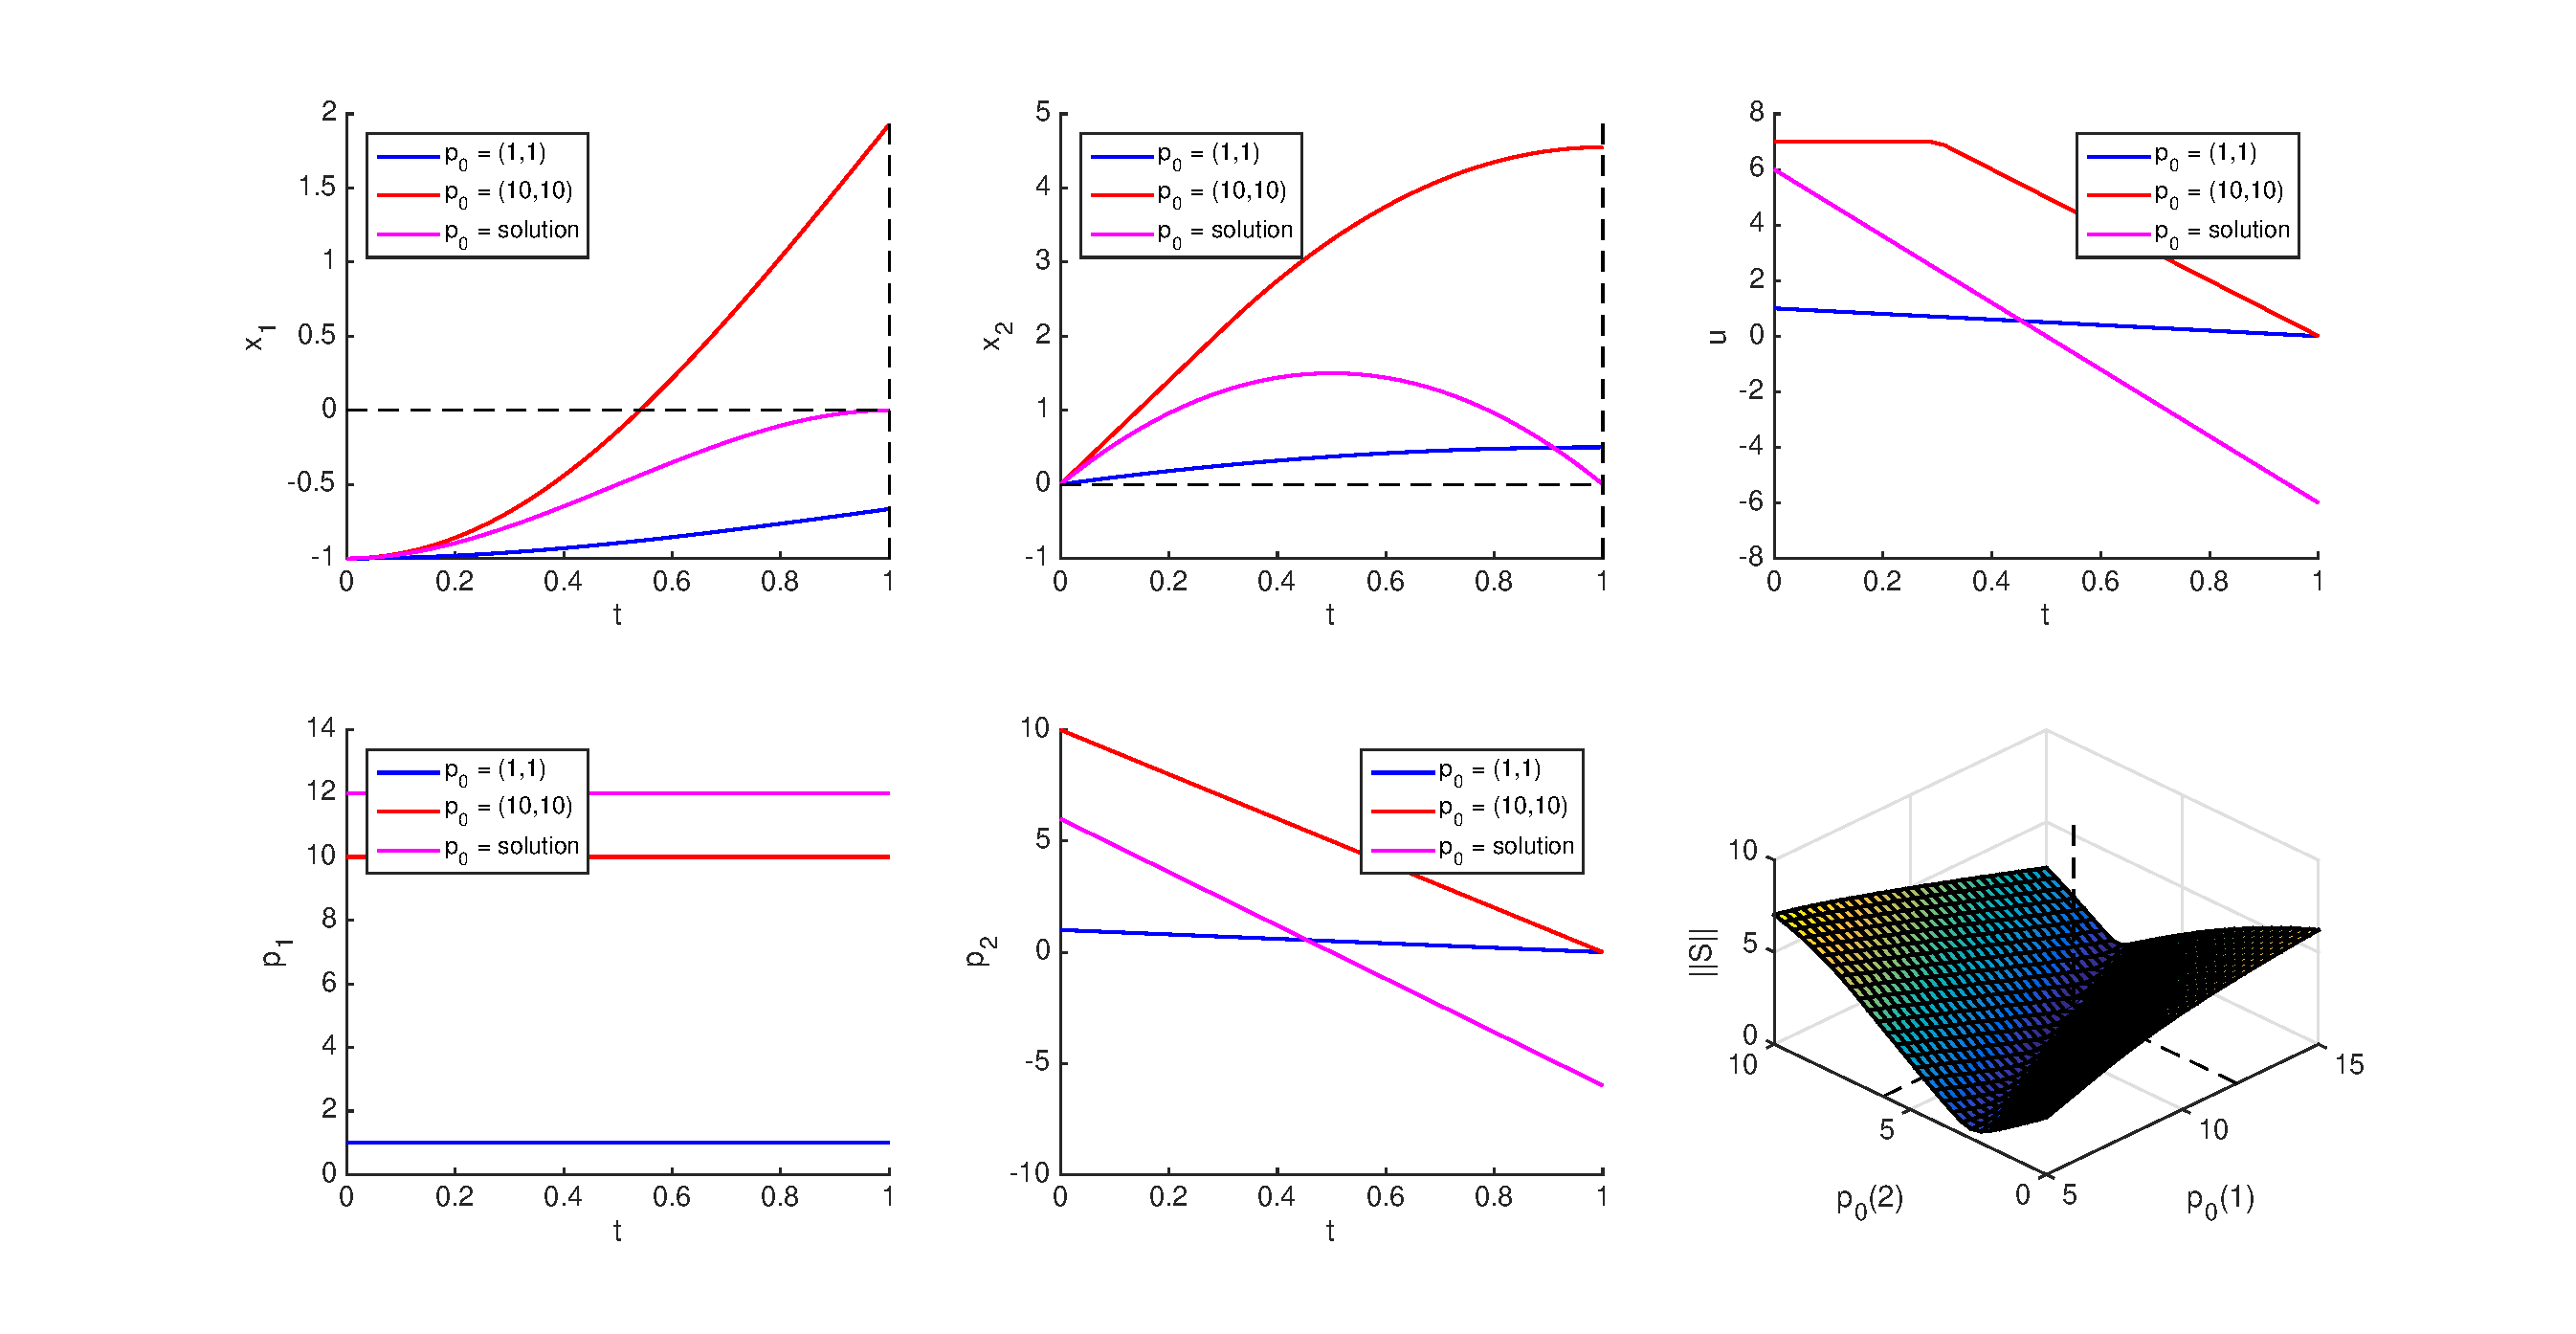
\includegraphics[width=0.99\textwidth]{results_tests_tir_simple_dim2}
    \end{center}
    \caption{R\'esultats apr\`es ex\'ecution du fichier \cmd{sujet1\_tir\_simple/probleme3/main.m}.}
    \label{fig:results_tests_tir_simple_dim2}
\end{figure}

\subsection{D\'efinition du probl\`eme}

Consid\'erons le probl\`eme de contr\^ole optimal suivant.
\leqnomode
\begin{equation}
\tagProblem
    \left\{ 
        \begin{array}{l}
            \displaystyle J(u(\cdot)) \coloneqq \displaystyle \frac{1}{2} \int_0^{t_f} u(t)^2 \, \diff t\longrightarrow \min            \\[1.0em]
            \dot{x}_1(t)    =  \displaystyle x_2(t)                                                                                     \\[0.5em]
            \dot{x}_2(t)    =  \displaystyle u(t), \quad \abs{u(t)} \le u_\mathrm{max}, \quad t \in \intervalleff{0}{t_f} \text{ p.p.}, \\[1.0em]
            x(0) = x_0 , \quad x(t_f) = x_f,
        \end{array}
    \right. 
    \label{eq:ocpSimpleDim2}
\end{equation}
\reqnomode
avec $t_f \coloneqq 1$, $x_0 \coloneqq (-1,0)$, $x_f \coloneqq (0,0)$ et $\forall\, t \in\intervalleff{0}{t_f}$, $x(t) = (x_1(t), x_2(t)) \in \R^2$.
Notons 
\[
    H(x,p,p^0,u) \coloneqq p_1\, x_2 + p_2\, u + p^0\, \frac{1}{2} u^2, \quad x = (x_1, x_2), \quad p = (p_1, p_2),
\]
le pseudo-hamiltonien associ\'e au probl\`eme \eqref{eq:ocpSimpleDim2}. On consid\`ere le cas normal et on fixe $p^0 = -1$. La condition de maximisation
nous donne comme loi de contr\^ole~:
\begin{equation}
    u(t) = 
    \left\{
        \begin{array}{ll}
            u_s(x(t),p(t)) \coloneqq p_2(t)   & \text{ si } \abs{p_2(t)} \le u_\mathrm{max}, \\[0.5em]
            +u_\mathrm{max}                      & \text{ si } p_2(t) > u_\mathrm{max}, \\[0.5em]
            -u_\mathrm{max}                      & \text{ si } p_2(t) < -u_\mathrm{max}.
        \end{array}
    \right.
    \label{eq:controleOCPSimpleDim2}
\end{equation}

\subsection{R\'esolution des \'equations de tir et influence de la borne sur le contr\^ole}

\begin{myExercice} R\'esolution des \'equations de tir.
    \begin{enumerate}
        \item Se rendre dans le r\'epertoire \cmd{sujet1\_tir\_simple/probleme3}.
        \item Impl\'ementer dans le r\'epertoire \cmd{lib} les fonctions \cmd{control}, \cmd{hvfun}, \cmd{exphvfun}, \cmd{sfun} et \cmd{ssolve},
            associ\'ees au probl\`eme \eqref{eq:ocpSimpleDim2}.
        \item Ex\'ecuter le script \cmd{main.m} et v\'erifier les r\'esultats. La solution des \'equations de tir $S(y) = 0$ ($y$ est ici le
            vecteur adjoint initial $p_0$) associ\'ees au probl\`eme \eqref{eq:ocpSimpleDim2} est $\psol_0 = (12, 6)$ pour $u_\mathrm{max} \ge 6$.
        \item Ex\'ecuter le script \cmd{main.m} avec $u_\mathrm{max} = 5$ et v\'erifier que $\psol_0 = (12.8977, 6.44364)$, et qu'il existe
            $0 \le t_1 \le t_2 \le t_f$ tels que la loi de commande solution $t \mapsto \usol(t)$ v\'erifie~:
            $\usol(t) = u_\mathrm{max}$ sur $\intervalleff{0}{t_1}$,
            $\usol(t) = u_s(\xsol(t),\psol(t))$ sur $\intervalleff{t_1}{t_2}$ et
            $\usol(t) = -u_\mathrm{max}$ sur $\intervalleff{t_2}{t_f}$.
    \end{enumerate}
\end{myExercice}

\begin{myremark}
    \anoter
    La loi de commande $\usol(\cdot)$ associ\'ee \`a la solution des \'equations de tir est lisse lorsque $u_\mathrm{max} \ge 6$.
    Pour $u_\mathrm{max} < 6$, la loi de commande perd en r\'egularit\'e. Pour $u_\mathrm{max} = 5$, elle est continue mais pas $C^1$,
    seulement $C^1$ par morceaux (elle est m\^eme lisse par morceaux).
\end{myremark}

\begin{myremark}
    \anoter
    On verra au sujet \ref{chap:tir_multiple_bang_bang} des lois de commande qui ne sont pas continues, mais toujours lisses par morceaux.
    Attention, dans ce cas l\`a, nous n'utiliserons plus une m\'ethode de tir simple mais de tir multiple pour r\'esoudre les \'equations de tir.
\end{myremark}

